\documentclass[11pt, a4paper]{article}

\usepackage[utf8]{inputenc}
\usepackage[T1]{fontenc}
\usepackage[a4paper, margin=2.5cm]{geometry}
\usepackage{enumitem}
\setlist[itemize]{label=-}
\usepackage{hyperref}
\usepackage{xurl}
\emergencystretch=3em
\usepackage{graphicx}
\usepackage{array}
\usepackage{booktabs}
\usepackage{amsmath}
\usepackage{xcolor}
\usepackage{listings}
\usepackage{pgfplots}
\pgfplotsset{compat=1.16}

\lstset{
  basicstyle=\ttfamily\footnotesize,
  breaklines=true,
  frame=single,
  columns=fullflexible,
  keepspaces=true,
  showstringspaces=false
}

% Captura de ecrã: usa o ficheiro se existir, senão mostra uma caixa
\newcommand{\figecra}[1]{%
  \IfFileExists{#1}%
    {\includegraphics[width=\linewidth]{#1}}%
    {\fbox{\parbox{0.92\linewidth}{\centering\vspace{1.4cm}%
      \texttt{\detokenize{#1}}\ (captura de ecrã por inserir)\vspace{1.4cm}}}}}

\title{\textbf{Análise e Redução do Volume de Tráfego do FACEIT (CS2): Captura Global, Classificação, Filtragem e Agregação em Fluxos}}
\author{
  \textbf{GRUPO 6} \\[0.4cm]
  Ivo Costa Sousa -- \texttt{pg63976} \\[0.15cm]
  João Afonso Almeida Sousa -- \texttt{pg62405} \\[0.15cm]
  João Carlos Teixeira Neiva -- \texttt{pg63978} \\[0.15cm]
}
\date{Novembro de 2026}

\begin{document}

\maketitle

\begin{abstract}
\textit{Este relatório, desenvolvido para a Unidade Curricular de Qualidade de Serviço na Internet, analisa o tráfego gerado pela plataforma FACEIT durante uma partida de CS2. A partir de uma captura global com o Wireshark (326\,122 pacotes, 206,9~MB, cerca de 30 minutos), o serviço é classificado num plano de jogo (um único fluxo UDP, 79\,\% dos bytes) e num plano de controlo (DNS, TLS e QUIC, cerca de 1\,\% do volume). São ainda estudados os critérios de filtragem mais eficazes e quantificada a redução de volume obtida por filtragem (21,3\,\%), truncagem de pacotes (87,5\,\%), \emph{sampling} combinado com truncagem (98,9\,\%) e agregação em fluxos com o Argus (até 99,97\,\%).}
\end{abstract}

\section{Parte 1: Objetivos e Metodologia}

\subsection{Objetivos}
Este trabalho consolida as etapas estudadas sobre captura e análise de tráfego, tendo como serviço de estudo o \textbf{FACEIT}, plataforma competitiva de partidas de CS2. Os objetivos definidos foram:
\begin{itemize}
    \item \textbf{Captura global:} Gerar tráfego real do serviço e capturar todo o tráfego da máquina com o Wireshark.
    \item \textbf{Classificação e filtragem:} Estudar os critérios mais eficazes, tanto em filtros de captura como em filtros de visualização.
    \item \textbf{Redução de volume:} Quantificar a percentagem de otimização face à captura global por filtragem, truncagem de pacotes e \textit{sampling}.
    \item \textbf{Agregação em fluxos:} Explorar uma ferramenta de agregação de pacotes em fluxos a partir de ficheiros \texttt{pcap}.
\end{itemize}

\subsection{Captura}
O Wireshark correu na própria máquina de jogo (\texttt{192.168.1.82}), ligada por cabo, \textbf{sem filtro de captura e com pacotes inteiros}, durante 1\,818,6~s (cerca de 30 minutos) e com o FACEIT Anti-Cheat ativo. Antes da captura final realizou-se um ensaio num servidor normal de CS2, fora do FACEIT, para validar o procedimento.

\subsection{Estratégia de Análise}
Optou-se por uma única captura global, convertida para \texttt{pcap} simples (\texttt{editcap -F pcap}) para servir de \textit{baseline}. Todos os cenários reduzidos foram \textbf{derivados offline desse mesmo ficheiro}, garantindo que a comparação incide exatamente sobre o mesmo tráfego. Recorreu-se ao Wireshark/\texttt{tshark}, \texttt{editcap}, \texttt{capinfos}, \texttt{tcpdump} e ao Argus.

A percentagem de otimização foi calculada, em bytes (tamanho do ficheiro) e em número de pacotes, por:
\[
  \text{redução} = \left(1 - \frac{\text{tamanho reduzido}}{\text{tamanho global}}\right)\times 100
\]
O tamanho do ficheiro inclui 16~B de cabeçalho por pacote no formato \texttt{pcap}. O campo \textit{Data size} do \texttt{capinfos} não reflete a truncagem, pelo que não foi utilizado.

\section{Parte 2: Caracterização do Tráfego}

\subsection{Visão Geral}
A captura global contém 326\,122 pacotes e 201,6~MB de dados (212,6~MB em \texttt{pcapng} e 206,9~MB em \texttt{pcap}), com uma média de 618~B por pacote e 179 pacotes/s. A composição por classe encontra-se na Tabela \ref{tab:comp}; as classes sobrepõem-se parcialmente, pelo que não devem ser somadas.

\begin{table}[hbt!]
\centering
\caption{Composição do Tráfego Global}
\label{tab:comp}
\begin{tabular}{@{} >{\raggedright\arraybackslash}p{6.2cm} r r r r @{}}
\toprule
\textbf{Classe} & \textbf{Pacotes} & \textbf{Bytes} & \textbf{\% Pacotes} & \textbf{\% Bytes} \\
\midrule
Servidor de jogo (\texttt{141.95.32.214})    & 202\,086 & 159\,679\,469 & 62,0 & 79,2 \\
UDP \texttt{:19336} (\texttt{104.29.146.69}) &  85\,785 &  17\,938\,347 & 26,3 &  8,9 \\
TCP (todo)                                    &  19\,394 &  12\,376\,258 &  5,9 &  6,1 \\
QUIC (todo)                                   &   7\,226 &   9\,622\,529 &  2,2 &  4,8 \\
mDNS / SSDP / DNS                             &   4\,576 &   1\,307\,245 &  1,4 &  0,6 \\
Controlo FACEIT (\texttt{193.41.200.101/102}) &   3\,995 &   3\,338\,873 &  1,2 &  1,7 \\
\bottomrule
\end{tabular}
\end{table}

\subsection{Plano de Jogo}
A conversa UDP \texttt{192.168.1.82:50088} $\leftrightarrow$ \texttt{141.95.32.214:27031} domina a captura (Figura \ref{fig:udp}). Inicia-se aos 293,8~s, dura 1\,520,5~s e totaliza 202\,006 pacotes e 159,7~MB. Os seus principais indicadores são:
\begin{itemize}
    \item \textbf{Sentido cliente $\rightarrow$ servidor:} 96\,786 pacotes (70,7~MB), com média de 730~B por pacote.
    \item \textbf{Sentido servidor $\rightarrow$ cliente:} 105\,220 pacotes (89,0~MB), com média de 846~B por pacote.
    \item \textbf{Débito:} Praticamente constante, com cerca de 133 pacotes/s e 0,84~Mbit/s (aproximadamente 40\,000 pacotes por cada 300~s).
    \item \textbf{Tamanho dos pacotes:} Concentrado entre 640 e 1\,279~B (69,3\,\% dos pacotes), com média de 790~B.
\end{itemize}

\subsection{Plano de Controlo}
O DNS e o SNI (em TLS e QUIC) permitem identificar inequivocamente o serviço. Foram observados os nomes \nolinkurl{www.faceit.com}, \nolinkurl{edge.faceit.com}, \nolinkurl{chat.faceit.com}, \nolinkurl{faceit.com}, \nolinkurl{cdn-frontend.faceit-cdn.net}, \nolinkurl{distribution.faceit-cdn.net} e \nolinkurl{ac-client-ws.faceit.com}, todos resolvidos para \texttt{193.41.200.101} e \texttt{193.41.200.102} (Figuras \ref{fig:sni} e \ref{fig:dns}), a que se junta \nolinkurl{analytics.faceitanalytics.com} (Cloudflare).

O primeiro contacto ocorre aos 2,2~s (QUIC para \nolinkurl{www.faceit.com}), surge uma nova rajada de pedidos entre os 225 e os 245~s, antes de o fluxo de jogo começar, e um último contacto a \nolinkurl{ac-client-ws.faceit.com} aos 1\,804,6~s. Este plano é reduzido: 3\,995 pacotes e 3,3~MB.

\subsection{Ruído}
Os fluxos UDP para \texttt{104.29.146.69:19336} (um novo fluxo por minuto, 85\,785 pacotes) são independentes do jogo, uma vez que surgiam também na captura de ensaio; a sua origem não foi identificada. O restante tráfego corresponde à rede local (mDNS, SSDP, \textit{broadcasts}) e a outras ligações HTTPS/QUIC.

\begin{figure}[hbt!]
\centering
\figecra{fig_udp.png}
\caption{\textit{Conversations} $\rightarrow$ UDP, ordenado por pacotes: o fluxo para \texttt{141.95.32.214:27031} domina.}
\label{fig:udp}
\end{figure}

\begin{figure}[hbt!]
\centering
\figecra{fig_sni.png}
\caption{Filtro \texttt{tls.handshake.extensions\_\allowbreak server\_name contains "faceit"} (TLS e QUIC).}
\label{fig:sni}
\end{figure}

\begin{figure}[hbt!]
\centering
\figecra{fig_dns.png}
\caption{Filtro \texttt{dns.qry.\allowbreak name contains "faceit"}.}
\label{fig:dns}
\end{figure}

\section{Parte 3: Critérios de Classificação e Filtragem}

\subsection{Filtros Estudados}
O filtro de captura (BPF) apenas tem acesso aos cabeçalhos (IP, protocolo, portas), pelo que critérios baseados em nomes (DNS/SNI) só são possíveis como filtros de visualização. A eficácia de cada critério foi avaliada através da \textbf{cobertura} (pacotes do jogo apanhados / pacotes do jogo) e da \textbf{precisão} (pacotes do jogo apanhados / pacotes apanhados), tomando como referência a conversa do jogo (202\,006 pacotes). Os resultados constam da Tabela \ref{tab:filtros}.

\begin{table}[hbt!]
\centering
\small
\caption{Critérios de Classificação e Respetiva Eficácia}
\label{tab:filtros}
\begin{tabular}{@{} >{\raggedright\arraybackslash}p{2.3cm} >{\raggedright\arraybackslash}p{4.1cm} >{\raggedright\arraybackslash}p{4.6cm} r r @{}}
\toprule
\textbf{Critério} & \textbf{Filtro de Captura (BPF)} & \textbf{Filtro de Visualização} & \textbf{Pacotes} & \textbf{Precisão} \\
\midrule
Servidor (IP) & \texttt{udp and host 141.95.32.214} & \texttt{ip.addr==141.95.32.214 \&\& udp} & 202\,006 & 100\,\% \\
\addlinespace
Qualquer protocolo com o IP & \texttt{host 141.95.32.214} & \texttt{ip.addr==141.95.32.214} & 202\,060 & 99,97\,\% \\
\addlinespace
Gama de portas & \texttt{udp portrange 27000-27050} & \texttt{udp.port>=27000 \&\& \allowbreak udp.port<=27050} & 202\,040 & 99,98\,\% \\
\addlinespace
Só UDP & \texttt{udp} & \texttt{udp} & 300\,571 & 67,2\,\% \\
\addlinespace
Controlo (IP) & \texttt{host 193.41.200.101 or \allowbreak host 193.41.200.102} & \texttt{ip.addr==193.41.200.101 \textbar\textbar{} \allowbreak ip.addr==193.41.200.102} & 3\,995 & --- \\
\addlinespace
Controlo (nome) & (não aplicável) & \texttt{dns.qry.\allowbreak name contains "faceit"}; \texttt{tls.handshake.\allowbreak extensions\_\allowbreak server\_name contains "faceit"} & --- & --- \\
\addlinespace
Jogo + controlo & \texttt{host} servidor \texttt{or host} controlo (2 IPs) & --- & 206\,055 & --- \\
\bottomrule
\end{tabular}
\end{table}

\subsection{Discussão}
Todos os filtros baseados em IP ou em portas atingem uma cobertura de 100\,\% do fluxo de jogo. A gama de portas apanha apenas 34 pacotes a mais do que o filtro por IP (precisão de 99,98\,\%) e tem a vantagem de não depender do IP do servidor, que muda de partida para partida. Em contrapartida, o filtro apenas por protocolo (\texttt{udp}) revela-se demasiado abrangente, já que 33\,\% do que apanha não pertence ao jogo.

Conclui-se que a deteção do fluxo de jogo é mais eficaz através da combinação de três critérios: transporte UDP, gama de portas \texttt{27xxx} e dominância por volume (\textit{Conversations} ordenado por bytes), sendo o serviço confirmado pelo DNS/SNI do plano de controlo.

\section{Parte 4: Redução de Volume}

\subsection{Resultados}
A Tabela \ref{tab:red} e a Figura \ref{fig:red} apresentam os cenários avaliados. Todas as percentagens são cumulativas face ao \textit{baseline} (A) de 326\,122 pacotes e 206\,864\,624~B.

\begin{table}[hbt!]
\centering
\small
\caption{Redução de Volume face à Captura Global}
\label{tab:red}
\begin{tabular}{@{} l >{\raggedright\arraybackslash}p{5.4cm} r r r r @{}}
\toprule
 & \textbf{Cenário} & \textbf{Pacotes} & \textbf{Bytes} & \textbf{Red. Bytes} & \textbf{Red. Pacotes} \\
\midrule
A  & Captura global (\textit{baseline})            & 326\,122 & 206\,864\,624 & 0\,\%     & 0\,\% \\
B1 & Filtro \texttt{udp and host} servidor         & 202\,006 & 162\,905\,309 & 21,25\,\% & 38,06\,\% \\
B3 & Filtro gama de portas 27000--27050            & 202\,040 & 162\,951\,481 & 21,23\,\% & 38,05\,\% \\
B4 & Filtro só \texttt{udp}                        & 300\,571 & 193\,613\,964 &  6,41\,\% &  7,83\,\% \\
B5 & Filtro jogo + controlo FACEIT                 & 206\,055 & 166\,312\,206 & 19,60\,\% & 36,82\,\% \\
\addlinespace
C1 & B1 + \textit{snaplen} 128                     & 202\,006 &  32\,311\,732 & 84,38\,\% & 38,06\,\% \\
C2 & B1 + \textit{snaplen} 96                      & 202\,006 &  25\,856\,584 & 87,50\,\% & 38,06\,\% \\
C3 & B1 + \textit{snaplen} 64                      & 202\,006 &  19\,392\,644 & 90,63\,\% & 38,06\,\% \\
C4 & B5 + \textit{snaplen} 96                      & 206\,055 &  26\,333\,772 & 87,27\,\% & 36,82\,\% \\
\addlinespace
D1 & B1 + \textit{sampling} 1/10                   &  20\,200 &  16\,376\,628 & 92,08\,\% & 93,81\,\% \\
D2 & B1 + \textit{snaplen} 96 + \textit{sampling} 1/10 & 20\,200 & 2\,262\,424 & 98,91\,\% & 93,81\,\% \\
\addlinespace
E1 & Fluxos Argus, global (registos de 5~s)        & --- &   1\,004\,872 & 99,51\,\% & --- \\
E2 & Fluxos Argus, global (1 registo/fluxo, CSV)   & --- &      64\,839 & 99,97\,\% & --- \\
E3 & Fluxos Argus, só servidor (CSV, 1 fluxo)      & --- &         229 & $\approx$100\,\% & --- \\
\bottomrule
\end{tabular}
\end{table}

\begin{figure}[hbt!]
\centering
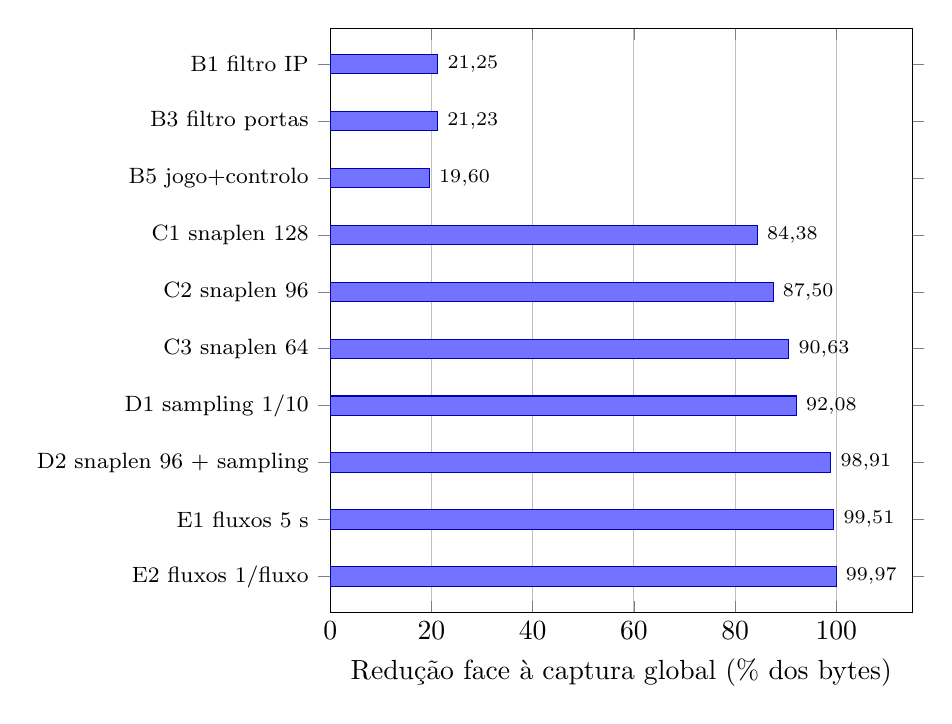
\begin{tikzpicture}
\begin{axis}[
  xbar, width=0.74\linewidth, height=9cm,
  xmin=0, xmax=115, xlabel={Redução face à captura global (\% dos bytes)},
  symbolic y coords={B1 filtro IP, B3 filtro portas, B5 jogo+controlo, C1 snaplen 128, C2 snaplen 96, C3 snaplen 64, D1 sampling 1/10, D2 snaplen 96 + sampling, E1 fluxos 5 s, E2 fluxos 1/fluxo},
  ytick=data, y dir=reverse, enlarge y limits=0.07, bar width=7pt,
  yticklabel style={font=\footnotesize}, xmajorgrids,
  nodes near coords={\pgfmathprintnumber[use comma,fixed,fixed zerofill,precision=2]{\pgfplotspointmeta}},
  every node near coord/.append style={font=\scriptsize}
]
\addplot[fill=blue!55,draw=blue!70!black] coordinates {
  (21.25,B1 filtro IP) (21.23,B3 filtro portas) (19.60,B5 jogo+controlo)
  (84.38,C1 snaplen 128) (87.50,C2 snaplen 96) (90.63,C3 snaplen 64)
  (92.08,D1 sampling 1/10) (98.91,D2 snaplen 96 + sampling)
  (99.51,E1 fluxos 5 s) (99.97,E2 fluxos 1/fluxo)};
\end{axis}
\end{tikzpicture}
\caption{Redução de Bytes por Cenário}
\label{fig:red}
\end{figure}

\subsection{Filtragem}
Filtrar o fluxo de jogo reduz apenas 21,25\,\% dos bytes, mas 38,06\,\% dos pacotes. Esta assimetria explica-se pelo facto de o jogo já representar 79\,\% dos bytes capturados, enquanto o ruído é composto por muitos pacotes pequenos: os 85\,785 pacotes de \texttt{:19336} correspondem a 26\,\% dos pacotes, mas a apenas 9\,\% dos bytes. Incluir o plano de controlo no filtro tem um custo reduzido (19,60\,\% contra 21,25\,\%) e descreve o serviço de forma mais completa.

\subsection{Truncagem de Pacotes (\textit{Snaplen})}
Não capturar o pacote inteiro é a técnica com maior impacto individual. Os cabeçalhos Ethernet, IPv4 e UDP ocupam 42~B, pelo que, com \textit{snaplen} 96, se preservam os cabeçalhos e mais 54~B de \textit{payload}. Com pacotes de 790~B em média, a redução total sobe de 21,25\,\% para 87,50\,\% (84,38\,\% com 128~B e 90,63\,\% com 64~B). O custo é a perda do restante \textit{payload}.

\subsection{\textit{Sampling}}
Guardar 1 pacote em cada 10 (por ordem de pacote) proporciona uma redução de 92,08\,\% sem truncagem e de 98,91\,\% com \textit{snaplen} 96 (2,26~MB, dos quais cerca de 0,32~MB correspondem a cabeçalhos de pacote do formato \texttt{pcap}). As estatísticas de volume mantêm-se fiáveis: extrapolando $\times 10$, o erro é de $-0{,}003\,\%$ nos pacotes e de $+0{,}54\,\%$ nos bytes. Perdem-se, contudo, as sequências de pacotes consecutivos.

\section{Parte 5: Agregação de Pacotes em Fluxos}

\subsection{Ferramenta e Processo}
Recorreu-se ao \textbf{Argus} (\texttt{argus -r f.pcap -w f.argus}), que emite registos de estado de cerca de 5~s por fluxo, e ao \texttt{racluster} para obter um único registo por fluxo (5-tuplo), exportado para CSV através do \texttt{ra}.

\subsection{Resultados}
A partir do \textit{baseline} de 206,9~MB obtiveram-se os seguintes volumes:
\begin{itemize}
    \item \textbf{Registos de 5~s:} 1,0~MB (redução de 99,51\,\%).
    \item \textbf{Um registo por fluxo (binário):} 122,7~kB (redução de 99,94\,\%).
    \item \textbf{Um registo por fluxo (CSV):} 64,8~kB (redução de 99,97\,\%), com 797 fluxos, mais um registo de gestão do Argus.
    \item \textbf{Apenas o servidor de jogo:} um único registo de 229~B no CSV.
\end{itemize}

Os totais do fluxo de jogo no Argus (70\,661\,525~B do cliente e 89\,011\,664~B do servidor) somam 159\,673\,189~B, exatamente o volume de dados do \texttt{pcap} filtrado. A agregação conserva o 5-tuplo, o instante de início, a duração e os pacotes e bytes por sentido, mas perde a temporização e o tamanho de cada pacote, bem como o \textit{payload}. Os registos de 5~s (E1) conservam ainda a evolução temporal do fluxo.

\section{Parte 6: Conclusões}

\subsection{Síntese}
\begin{itemize}
    \item \textbf{Estrutura do serviço:} O tráfego do FACEIT divide-se num plano de jogo (UDP \texttt{141.95.32.214:27031}, 79\,\% dos bytes) e num plano de controlo (DNS/TLS/QUIC para \texttt{193.41.200.101/102}, cerca de 1\,\%).
    \item \textbf{Classificação:} Os critérios mais eficazes para detetar o fluxo de jogo são o transporte UDP, a gama de portas \texttt{27000--27050} e a dominância por volume; o DNS/SNI confirma o serviço. O filtro apenas por protocolo é demasiado abrangente.
    \item \textbf{Redução de volume:} A filtragem poupa pouco em bytes (21\,\%), dado que o jogo domina a captura. As maiores poupanças resultam do \textit{snaplen} (87,5\,\%), do \textit{sampling} (98,9\,\% em conjunto) e da agregação em fluxos (99,5\,\% a 99,97\,\%).
    \item \textbf{Escolha da técnica:} Depende da utilização pretendida: cabeçalhos por pacote $\Rightarrow$ filtro e \textit{snaplen} 96; estatísticas de volume $\Rightarrow$ \textit{sampling}; contabilização e retenção prolongada $\Rightarrow$ fluxos.
\end{itemize}

\subsection{Limitações}
Foi analisada uma única captura de uma única partida, e o IP e a porta do servidor mudam entre partidas. Os cenários foram derivados offline da captura global, e não capturados ao vivo. O \textit{sampling} aplicado é determinístico (1 em 10 por ordem de pacote) e as percentagens em ficheiro incluem o cabeçalho de 16~B por pacote do formato \texttt{pcap}. Por fim, apenas o Argus foi utilizado para a agregação em fluxos.

\appendix
\section{Comandos Utilizados}
\begin{lstlisting}
# Baseline
capinfos faceit.pcapng
editcap -F pcap faceit.pcapng A_global.pcap

# Caracterizacao
tshark -r A_global.pcap -q -z io,phs
tshark -r A_global.pcap -q -z conv,udp
tshark -r A_global.pcap -q -z plen,tree,"ip.addr==141.95.32.214"
tshark -r A_global.pcap -Y 'dns.flags.response==1 && dns.qry.name contains "faceit"' -T fields -e frame.time_relative -e dns.qry.name -e dns.a
tshark -r A_global.pcap -Y 'tls.handshake.extensions_server_name contains "faceit"' -T fields -e frame.time_relative -e ip.dst -e tls.handshake.extensions_server_name

# Filtros (BPF, aplicados offline)
tcpdump -r A_global.pcap -w B1_udp_host.pcap  "udp and host 141.95.32.214"
tcpdump -r A_global.pcap -w B3_portrange.pcap "udp portrange 27000-27050"
tcpdump -r A_global.pcap -w B4_udp.pcap       "udp"
tcpdump -r A_global.pcap -w B5_game_ctrl.pcap "host 141.95.32.214 or host 193.41.200.101 or host 193.41.200.102"

# Snaplen e sampling
editcap -s 96 B1_udp_host.pcap C2_snaplen96.pcap
tshark -r C2_snaplen96.pcap -Y "frame.number % 10 == 0" -F pcap -w D2_snaplen_sampling.pcap

# Fluxos (Argus)
argus -r A_global.pcap -w E1_global.argus
racluster -r E1_global.argus -m proto saddr sport daddr dport -w E2_global_cluster.argus
ra -r E2_global_cluster.argus -n -c , -s stime dur proto saddr sport daddr dport spkts dpkts sbytes dbytes > E2_global_flows.csv

# Medicao
capinfos -T -m -M -c -s *.pcap
\end{lstlisting}

\end{document}
